\label{sec:mcnp}
\section{MCNP}
\subsection{General information}
MCNP is based on Fortran, the most common version being Fortran-90. The basic programming principle is similar to that of punch cards: a program is split into several blocks, where various aspects of a simulation are defined. The first block defines cells, the second one defines surfaces, finally, the last block defines what simulations MCNP is supposed to run. An example MCNP program structure can be seen in figure \ref{fig:program}. The blocks are separated by blank lines, which are required for MCNP to properly read in the file. If the lines are omitted, then the definitions will not be seen correctly. Comments can be added to the input files as well. A full line comment starts with the letter "c", whilst an inline comment starts with a dollar sign (\$). It is important to note that all lines should not exceed 80 characters in length.

\begin{figure}[!htbp]
\caption{MCNP program structure.}
\label{fig:program}
\centering
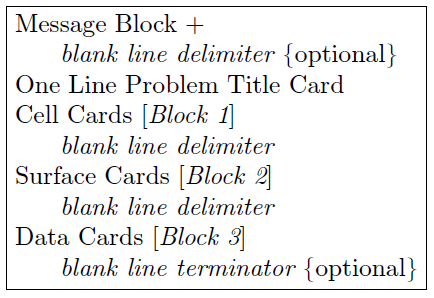
\includegraphics[width=0.5\textwidth]{prog.png}
\end{figure}

MCNP programs contain definitions for geometries in a 3D dimensional Cartesian coordinate system. A good way to look at cells, surfaces and their material definitions is the following. In figure \ref{fig:regions}, A and B are two surfaces. Each surface has a negative and positive value, which is important for particle interactions. If a value is negative, then the surface is facing inwards relative to the origin. The mathematical depiction can be seen in figure \ref{fig:planes}, where the normal vector $n_2$ is expressed by a negative surface number, whilst the vector $n_1$ is a positive surface number.

\begin{figure}[!htbp]
\caption{Normal vectors to a plane.}
\label{fig:planes}
\centering
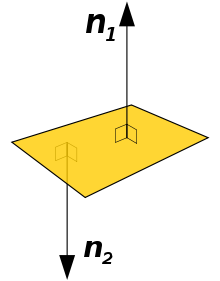
\includegraphics[width=0.25\textwidth]{normals.png}
\end{figure}

Surfaces can be combined together to create cells. Defined as either unions or intersections, the resulting cells from surfaces A and B are seen in figure \ref{fig:regions}. An important MCNP concept to remember is that when looking at a typical geometrical shape, for example a cube, one must double the number of faces. In a cube, the number of faces is 6, however, because of positive and negative surfaces, the shape should be looked at as having 12 faces\footnote{Similarly, a sphere will have 2 surfaces - an inner one and an outer one.}. Understanding this was a key point in the project. Being able to identify which regions were required and which surfaces to ignore allowed us to carry out simulations more effectively and accurately.

\begin{figure}[!htbp]
\caption{Example MCNP regions.}
\label{fig:regions}
\centering
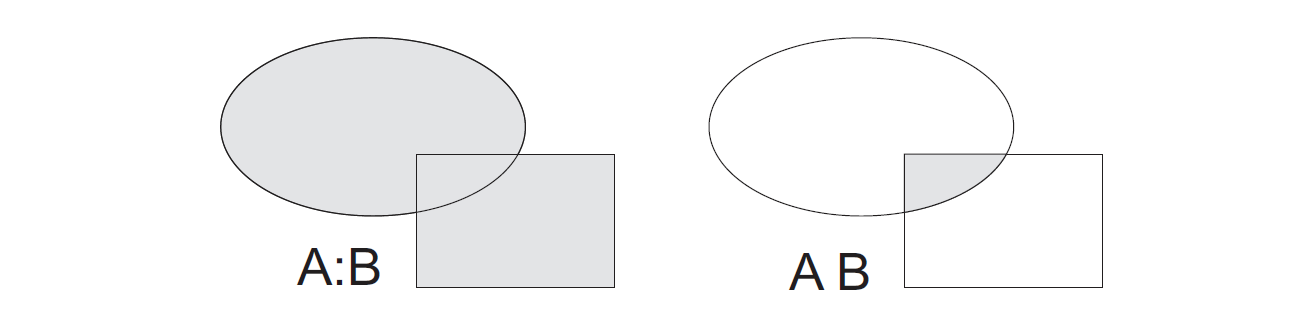
\includegraphics[width=0.75\textwidth]{regions.png}
\end{figure}

\subsection{Example geometry}

A good way to understand MCNP syntax and its complexity is a simple example. For this, a graphite cube will be submerged into a spherical container and that container will be filled with water. Throughout the project, it was found that specifying surfaces first was an easier approach, followed by the cell definitions. The input file was structured out of order, however, this allowed for a more step-by-step approach to the simulation setup. In order to create a cube, the procedure is the following:

\begin{enumerate}
	\item Specify 6 outward facing surfaces.
	\item Specify 6 inward facing surfaces.
	\item Combine all of the relevant surfaces into a cell. Here, the outside of the cube would be a union of the outward facing surfaces, and the inside will be a union of the inward facing ones.
\end{enumerate}

Although this is only 3 steps, the procedure is fairly complex. In order to specify a single surface, one must figure out the side length, center and boundaries of the square in question. Doing this 12 times becomes monotone and challenging, especially when dealing with complex, irregular geometries. MCNP does have a solution, however - macrobodies. With one command, MCNP will know that the shape specified is a cube, sphere or pyramid, to name a few. The command for a rectangular parallelepiped is \textbf{RPP}. In order to create a cube centered at the origin with a side length of $10$cm, the command is:

\begin{center}
\begin{tabular}{c}
\begin{lstlisting}
10 RPP -5 5 -5 5 -5 5
\end{lstlisting}
\end{tabular}
\end{center}

In the above example, 10 is the number of the macrobody, which will be important in the cell block - it is an identifier. The first two numbers indicate a starting and ending x-coordinate\footnote{MCNP units are metric, with length defaulting to centimeters.}, followed by the same syntax for y and z coordinates. The next step is to add a container around the cube. This can be a sphere, again, specified by a macrobody, the command for which is \textbf{SO}. If the radius is to be 100cm, then:

\begin{center}
\begin{tabular}{c}
\begin{lstlisting}
20 SO 100
\end{lstlisting}
\end{tabular}
\end{center}

The structure is similar - 20 is the label for the macrobody, SO is the command, 100 is the radius. For this example, we need water and graphite as the materials. These are specified in the final, data block. Material definitions are fairly straightforward. To label a material, one types the letter "M", followed by a number. After that, the material is defined by elemental and atomic abundances. Water, having 2 hydrogen atoms and an oxygen atom, is defined as:

\begin{center}
\begin{tabular}{c}
\begin{lstlisting}
M1 1000 2
   8000 1
\end{lstlisting}
\end{tabular}
\end{center}

The general format for isotope specification is $ZZZAAA$, where $ZZZ$ is the atomic number and $AAA$ is the mass number. Specifying $AAA$ as 000 tells MCNP to use the elemental form, as is done above. The 1000 and 8000 specify the forms of hydrogen and oxygen, respectively. To specify graphite, the label can be M2, with the atomic and mass numbers being equal to 12 and 60, respectively. To specify 100\% composition, we define graphite as\footnote{The 1 at the end of the command specifies fractional composition - 1 being equal to 100\%.}:

\begin{center}
\begin{tabular}{c}
\begin{lstlisting}
M2 06012 1
\end{lstlisting}
\end{tabular}
\end{center}

Since the surfaces and the materials have been defined, the cells' block can be examined now. The syntax is similar to previous definitions - a cell number, followed by its material, its density, surface number (positive or negative facing) and its importance. The density sign should match the surface number sign - if a surface is defined by a negative cell, then the density\footnote{Density is specified in terms of MCNP's constants - found either in the manual or primer.} will be negative as well. The importance is a property of the material to interact with particles. In this project's case, setting \text{imp:N=1} means that this cell will only interact with neutrons. Below is the definition for the graphite cube cell:

\begin{center}
\begin{tabular}{c}
\begin{lstlisting}
1 2 -1.7 -10 imp:N=1
\end{lstlisting}
\end{tabular}
\end{center}

The above definition completely sets up the cube at the center of the universe. In order to setup the surrounding water, the definition is presented below:

\begin{center}
\begin{tabular}{c}
\begin{lstlisting}
2 1 1 (10 -20) imp:N=1
\end{lstlisting}
\end{tabular}
\end{center}

The setup is the same as for the previous cell - its label is 2, M1 is used for the material (water), and the cell is defined as the union of the outward facing surfaces of the cube, but the inward facing surfaces of the sphere. The water will interact with the neutrons only. The setup is almost complete, however, the graveyard must be added. This is the boundary of the simulation where the particles simply vanish. To do this, the outward facing surface of the sphere has to be set to 0 importance and material 0, which is vacuum:

\begin{center}
\begin{tabular}{c}
\begin{lstlisting}
3 0 20 imp:N=0
\end{lstlisting}
\end{tabular}
\end{center}

The setup is complete and the full file can be found in the Appendix. Assuming you have saved the file as \textbf{example.txt}, there are several ways to run the program. The commands depend on your operating system, but primarily the version of MCNP used:

\begin{center}
\begin{tabular}{c}
\begin{lstlisting}
mcnp example.txt
mcnp6.mpi ir inp=example.txt
\end{lstlisting}
\end{tabular}
\end{center}

Since the data block does not have any simulation specifications (only the material definitions), MCNP will not output anything meaningful. In the second version of the command above, the flag "ir" was used to specify that the file should be run. In order to inspect the geometry and see if it is valid (assuming you have the graphical MCNP geometry editor), the flag "i" should be used by itself.

\label{sec:simulations}
\subsection{Data block}

\textbf{Criticality tests}\\

The final data block is where the simulation specifications, as well as other aspects like unit conversions are defined. In Layman's terms, this is where one tells MCNP what to do with the provided geometry. Two main types of simulations were run for the project - a criticality tests and an FMESH tally. The criticality test takes a fissionable source and sees if the geometry will be able to sustain the reaction. The value returned is called the k-coefficient. If the value is greater than 1, then the geometry (mainly the fissionable core that is being tested) is super critical. If it is equal to 1, then the setup is critical. Anything under 1 is non-critical and will die out. A typical criticality test is run using two commands: \textbf{kcode} and \textbf{ksrc}. The first command specifies the number of particle histories to look at, the k-coefficient value to attempt to obtain, number of cycles and samples. An example command is seen below:

\begin{center}
\begin{tabular}{c}
\begin{lstlisting}
kcode 1000  1.0  15 115
\end{lstlisting}
\end{tabular}
\end{center}

The above line indicates that 1000 particles will be looked at to attempt to obtain a criticality value of 1, with 115 samples and 15 cycles per sample. The only thing left to do is to specify the source of the reactions, in this case the origin:

\begin{center}
\begin{tabular}{c}
\begin{lstlisting}
ksrc 0 0 0
\end{lstlisting}
\end{tabular}
\end{center}

The k-code will emit particles from the source into a random direction and see if they trigger other fission reactions. This procedure links back to the random walk problem - every interaction a particle has with something else in the defined geometry is randomly generated/processed. After running for the specified number of samples, MCNP will output the criticality that results from the specified geometry. The results returned are in the forms of confidence intervals, however, the average value is the one to look at, which MCNP will also give you. This was the main approach to determining the size and composition of the core. Obtaining a value as close to $k=1$ was crucial for the GOFR since a runaway reaction would cause safety concerns. On the other hand, a sub-critical core would die out and the beam of neutrons emitted will not last long (or be powerful enough).

\textbf{FMESH tally}\\